\documentclass[11pt,a4paper]{article}
\usepackage[margin=2.3cm]{geometry}
\usepackage[T1]{fontenc}
\usepackage{mathptmx}
\renewcommand{\ttdefault}{pcr}
\usepackage{amsmath,amssymb,amsthm}
\usepackage{booktabs,tabularx,array,multirow}
\usepackage{graphicx}
\usepackage{subcaption}
\usepackage{caption}
\usepackage{float}
\usepackage{enumitem}
\usepackage{xcolor}
\usepackage{tikz}
\usetikzlibrary{arrows.meta,positioning,calc,decorations.pathreplacing,shapes.geometric,fit,backgrounds}
\usepackage{algorithm}
\usepackage[noend]{algpseudocode}
\usepackage[hidelinks]{hyperref}
\usepackage[nameinlink]{cleveref}
\urlstyle{same}
\setlist{itemsep=2pt,topsep=4pt}
\captionsetup{font=small,labelfont=bf}
\renewcommand{\arraystretch}{1.2}
\newcolumntype{L}{>{\raggedright\arraybackslash}X}
\newtheorem{lemma}{Lemma}

\definecolor{male}{HTML}{3498DB}
\definecolor{maleD}{HTML}{1B4F72}
\definecolor{female}{HTML}{E91E63}
\definecolor{femaleD}{HTML}{880E4F}
\definecolor{keep}{HTML}{27AE60}
\definecolor{greedy}{HTML}{C0392B}
\definecolor{hot}{HTML}{E67E22}
\definecolor{cyc}{HTML}{16A085}
\definecolor{grey}{HTML}{95A5A6}

\newcommand{\dirv}[1]{\mathbf{e}_{#1}}
\newcommand{\len}{\ell}
\newcommand{\Score}{\operatorname{score}}

\title{\textbf{The Family Metro Map Layout for General Graphs}\\[2pt]
\large Spanning tree, metro routing of cycle edges, overlap repair and complexity}
\author{Technical description of \texttt{family\_metro\_map\_graph.js}\\
(companion to the document on the tree algorithm, \texttt{familymetromap.js})}
\date{}

\begin{document}
\maketitle

\begin{abstract}
\noindent This document describes how the application draws an arbitrary undirected graph (cycles and several components allowed) with at most eight neighbours per vertex as a London-Underground-style metro map. Every edge runs along one of the eight octilinear directions and is either straight or has exactly one $45^\circ$ bend, and the edges at a vertex leave in different directions. The graph is split into a breadth-first spanning forest, whose edges are placed by the beam search of the tree algorithm, and the remaining \emph{cycle edges}, which are routed as metro links at the moment their second endpoint is placed. Because the cost of these routes is part of the placement score, vertices are placed where their cycles can close without crossings. A search over layout settings, overlap detection (incremental in step-by-step mode) and the Fix buttons complete the method. We state the constraints on the input (degree, self-loops, planarity), give every quantity used by the code, analyse the running time, and report experiments on grids, cycles, trees with extra edges, random graphs and $K_5$.
\end{abstract}

\setcounter{tocdepth}{1}
\tableofcontents
\bigskip

%==========================================================================
\section{Overview}

The input is an undirected graph $G=(V,E)$ with $n=|V|$ vertices, $m=|E|$ edges and $c$ connected components, a chosen root $r$, a shrinking factor $\alpha\in(0,1]$, and a gender $\sigma(v)\in\{\mathrm F,\mathrm M\}$ for every vertex (derived from the vertex label: an even character code of the first letter means female). The output is a position for every vertex and at most one bend point for every edge.

\begin{figure}[ht]
\centering
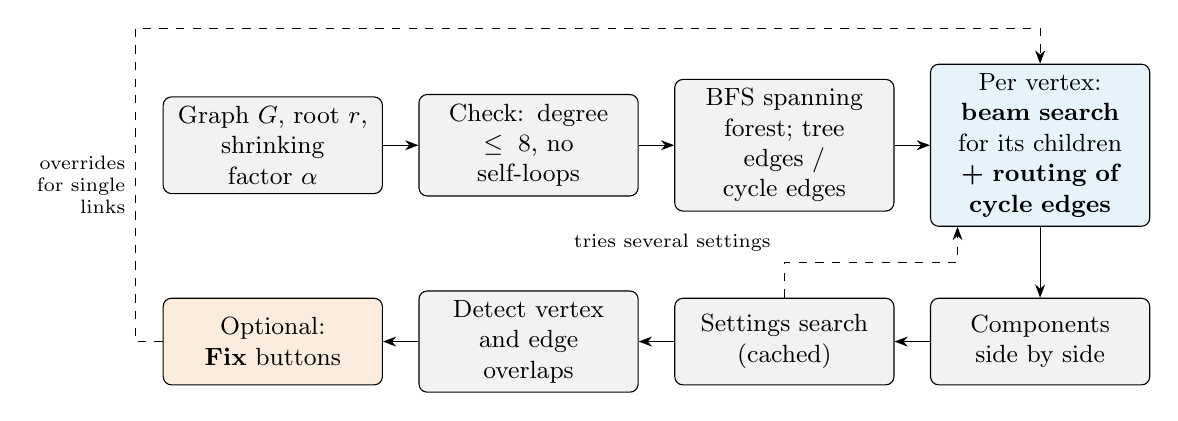
\begin{tikzpicture}[
  box/.style={draw, rounded corners=3pt, align=center, font=\small, minimum height=1.1cm, text width=2.55cm, fill=#1,
              execute at begin node=\hyphenpenalty 10000\relax},
  box/.default=white, >=Stealth, node distance=0.45cm]
\node[box=gray!10] (in) {Graph $G$, root $r$,\\ shrinking factor $\alpha$};
\node[box=gray!10, right=of in] (chk) {Check: degree\\ $\le 8$, no\\ self-loops};
\node[box=gray!10, right=of chk] (bfs) {BFS spanning\\ forest; tree\\ edges / cycle edges};
\node[box=male!12, right=of bfs] (beam) {Per vertex: \textbf{beam search} for its children \textbf{+ routing of cycle edges}};
\node[box=gray!10, below=0.9cm of beam] (pack) {Components\\ side by side};
\node[box=gray!10, left=of pack] (search) {Settings search\\ (cached)};
\node[box=gray!10, left=of search] (detect) {Detect vertex\\ and edge\\ overlaps};
\node[box=hot!15, left=of detect] (fix) {Optional:\\ \textbf{Fix} buttons};
\draw[->] (in) -- (chk); \draw[->] (chk) -- (bfs); \draw[->] (bfs) -- (beam);
\draw[->] (beam) -- (pack); \draw[->] (pack) -- (search); \draw[->] (search) -- (detect); \draw[->] (detect) -- (fix);
\draw[->, dashed] (search.north) -- ++(0,0.45) -| ($(beam.south west)+(0.35,0)$);
\node[font=\scriptsize, anchor=south east] at ($(search.north)+(-0.05,0.47)$) {tries several settings};
\draw[->, dashed] (fix.west) -- ++(-0.35,0) |- node[pos=0.25, left, font=\scriptsize, align=right]{overrides\\ for single\\ links} ($(beam.north)+(0,0.45)$) -- (beam.north);
\end{tikzpicture}
\caption{Pipeline. The layout (blue) is deterministic. The settings search and the Fix buttons never move vertices directly: they choose parameters or record \emph{overrides} for single links and re-run the layout, so cycle edges are always re-routed consistently.}
\label{fig:pipeline}
\end{figure}

\Cref{fig:grid5} shows a typical result. Edges of the spanning tree (grey) are drawn exactly as in the tree algorithm; cycle edges (green, dashed in all figures of this document; in the application all edges have the same colour) are metro links between two already placed vertices.

\begin{figure}[ht]
\centering
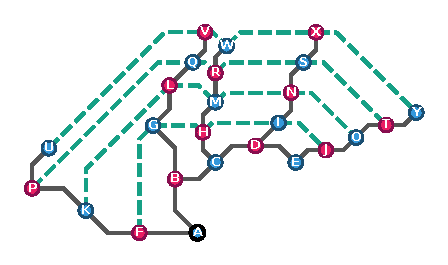
\includegraphics[width=0.42\textwidth]{fig_grid5.pdf}
\caption{A $5\times5$ grid graph ($n=25$, $m=40$, 16 cycle edges), root A (black border), $\alpha=0.75$. Grey: BFS spanning tree; green dashed: cycle edges. No vertex overlaps and no colliding edges.}
\label{fig:grid5}
\end{figure}

%==========================================================================
\section{Input and constraints}
\label{sec:constraints}

\begin{center}\small
\begin{tabularx}{\textwidth}{@{}l l L@{}}
\toprule
property & allowed? & remark\\
\midrule
cycles & yes & drawn as metro links (\cref{sec:cycle})\\
several components & yes & laid out separately and placed side by side (\cref{sec:components})\\
isolated vertices & yes & a component with one vertex\\
degree $\deg(v)\le 8$ & \textbf{required} & checked before every layout; otherwise an error names the vertices\\
self-loops & no & rejected (a loop cannot be drawn as a metro link)\\
parallel edges & no & the input formats (adjacency list / matrix) cannot express them\\
planarity & not required & but non-planar graphs always keep crossings (\cref{sec:planarity})\\
\bottomrule
\end{tabularx}
\end{center}

\subsection{Why at most eight neighbours}

A metro map has eight directions $k\cdot45^\circ$, $k=0,\dots,7$, and two edges that leave a vertex in the same direction share their first segment, which is reported as an edge overlap. A vertex can therefore have at most eight edges without a forced overlap. For a non-root vertex one direction is taken by the edge from its BFS parent, leaving seven for the remaining edges; the root has all eight available. The bound is necessary but not sufficient: the direction of a cycle edge is dictated by the positions of its endpoints (\cref{sec:shapes}), so two cycle edges can still compete for the same direction even when $\deg(v)\le 8$. Such conflicts are penalised during placement and are the target of the Fix buttons; when they cannot be removed they are reported.

\subsection{Planarity}
\label{sec:planarity}

The algorithm does \emph{not} test planarity and works for every graph that satisfies the degree bound. Planarity matters for what can be achieved:
\begin{itemize}
  \item A \textbf{non-planar} graph, for example $K_5$ or $K_{3,3}$, cannot be drawn without crossings in any style; at least its crossing number $\operatorname{cr}(G)$ of crossings remains ($\operatorname{cr}(K_5)=\operatorname{cr}(K_{3,3})=1$). These crossings appear in the Overlapping / Touching Edges panel and cannot be removed by the Fix buttons.
  \item A \textbf{planar} graph has a crossing-free straight-line drawing (F\'ary's theorem), but the metro style restricts the drawing much more: octilinear segments, at most one bend per edge, distinct directions at each vertex, and tree edges with gender-dependent shapes and prescribed lengths. The algorithm is a heuristic and does not guarantee a crossing-free result for every planar graph. In the experiments (\cref{sec:experiments}) all grids and cycles were drawn without any overlap.
  \item The method also does not aim for the minimum number of crossings, which is NP-hard to compute in general; it reduces collisions greedily and through the settings search and the Fix buttons.
\end{itemize}

\Cref{fig:k} contrasts the planar $K_4$ with the non-planar $K_5$.

\begin{figure}[ht]
\centering
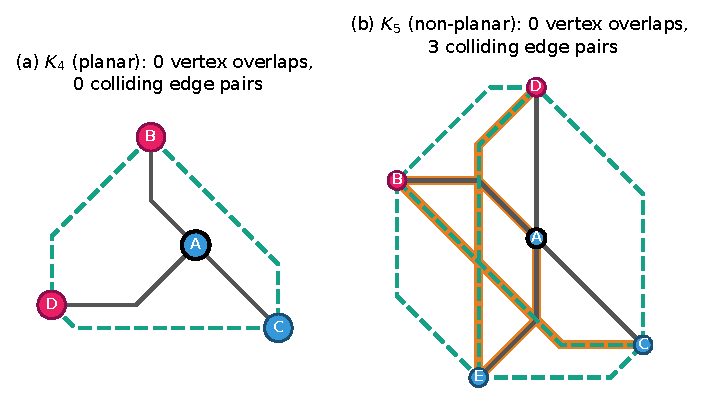
\includegraphics[width=0.7\textwidth]{fig_k.pdf}
\caption{Complete graphs ($\alpha=0.75$). (a) $K_4$ is planar and is drawn without collisions. (b) $K_5$ is not planar, so crossings cannot be avoided; colliding edges are highlighted in orange (here 3 colliding edge pairs, against the theoretical minimum of one crossing for $K_5$).}
\label{fig:k}
\end{figure}

%==========================================================================
\section{Spanning forest and tree edges}
\label{sec:tree}

\paragraph{Spanning forest.} A breadth-first search from the root $r$ visits its component and fixes, for every vertex $v\neq r$, a BFS parent $p(v)$; every other component is searched from its first vertex in input order. The \emph{tree edges} $\{v,p(v)\}$ form a spanning forest with $n-c$ edges; the remaining
\[
  k \;=\; m-n+c
\]
edges are the \emph{cycle edges}. BFS keeps cycle edges short in terms of generations: the endpoints of a cycle edge are in the same or in neighbouring BFS layers, so they are usually drawn close to each other.

\paragraph{Tree edges.} Tree edges are placed exactly as in the tree algorithm (see the companion document). Briefly: each vertex $v$ has an orientation $k(v)\in\{0,\dots,7\}$, even for female and odd for male vertices. The link $p(v)\to v$ leaves $p(v)$ in direction $(k(p(v))+g)\bmod 8$ with branch offset $g\in\{0,\pm2,\pm1,\pm3,4\}$; it is straight if that direction has the right parity for $v$ and otherwise has one $45^\circ$ bend $s=\pm1$ with two segments of length $\len/\sqrt{2+\sqrt2}$. The length is $\len=\max(L_0\,\alpha^{\gamma(v)},\,34\text{ px})$ with the line generation $\gamma$. Vertices are processed in BFS order, and the links to all children of a vertex are chosen together by a beam search of width $B$ (4 by default). A candidate is scored by
\[
  \Score_{\text{tree}} = 10^6 V + 10^5 E + 40\max(0,\,0.9\len-c) + P_{\text{room}} + 12\,\pi(g) - 0.02\,\bar\delta ,
\]
with vertex conflicts $V$, edge conflicts $E$, clearance $c$, look-ahead room $P_{\text{room}}$, branch preference $\pi(g)$ and average distance $\bar\delta$. The general-graph version adds two terms to this score (\cref{sec:beam}) and reserves the directions used by cycle edges (\cref{sec:ports}). If the graph is a tree there are no cycle edges, both additions vanish, and the layout is identical to the one of the tree algorithm (verified on 378 test trees, including trees with more than 100 vertices).

%==========================================================================
\section{Cycle edges as metro links}
\label{sec:cycle}

\subsection{Shapes}
\label{sec:shapes}

A cycle edge joins two vertices $w$ and $v$ that are both placed when it is routed, so its shape is determined by the vector $\mathbf d=p_v-p_w=(d_x,d_y)$. The direction of $\mathbf d$ lies in a $45^\circ$ sector between two neighbouring metro directions $d_1=\lfloor \operatorname{atan2}(d_y,d_x)/(\pi/4)\rfloor \bmod 8$ and $d_2=d_1+1 \bmod 8$. Writing $\mathbf d$ in the basis $\dirv{d_1},\dirv{d_2}$,
\[
  \mathbf d = s_1\,\dirv{d_1} + s_2\,\dirv{d_2},\qquad
  s_1=\frac{d_x e_{2,y}-d_y e_{2,x}}{\det(\dirv{d_1},\dirv{d_2})},\qquad
  s_2=\frac{e_{1,x}d_y-e_{1,y}d_x}{\det(\dirv{d_1},\dirv{d_2})},\qquad s_1,s_2\ge 0,
\]
with $\det(\dirv{d_1},\dirv{d_2})=\sin45^\circ$. This gives exactly two metro shapes with one bend (\cref{fig:shapes}):
\begin{itemize}
  \item \textbf{shape A:} first $s_1$ along $d_1$, then $s_2$ along $d_2$; bend at $p_w+s_1\dirv{d_1}$;
  \item \textbf{shape B:} first $s_2$ along $d_2$, then $s_1$ along $d_1$; bend at $p_w+s_2\dirv{d_2}$.
\end{itemize}
Both turn by $45^\circ$ (interior angle $135^\circ$), as on the London Underground map, and both have length $s_1+s_2$. If $\min(s_1,s_2)<1$\,px the second segment would be invisible, and the edge is drawn \textbf{straight} along the dominant direction. No other shapes are used: no right angles, no acute angles and never more than one bend.

The \emph{ports} of a shape are the directions in which it leaves its endpoints: shape A leaves $w$ in direction $d_1$ and arrives at $v$ in direction $d_2$, i.e.\ it occupies port $d_1$ at $w$ and port $(d_2+4)\bmod 8$ at $v$; for shape B the roles of $d_1$ and $d_2$ are swapped.

\begin{figure}[ht]
\centering
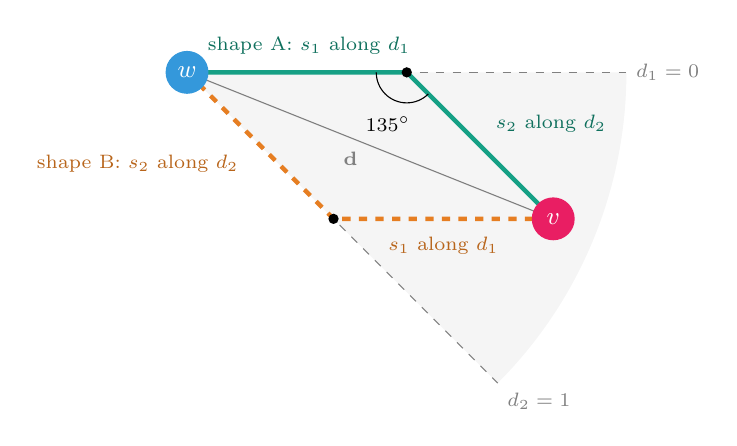
\begin{tikzpicture}[yscale=-1, scale=1.55, >=Stealth]
\coordinate (w) at (0,0); \coordinate (v) at (3,1.2);
\coordinate (A) at (1.8,0); \coordinate (B) at (1.2,1.2);
% sector
\fill[gray!8] (w) -- (3.6,0) arc (0:45:3.6) -- cycle;
\draw[gray, dashed] (w) -- (3.6,0) node[right, font=\scriptsize]{$d_1=0$};
\draw[gray, dashed] (w) -- (45:3.6) node[below right, font=\scriptsize]{$d_2=1$};
\draw[gray, ->, thin] (w) -- (v);
\node[font=\scriptsize, gray] at ($(w)!0.42!(v)+(0.08,0.2)$) {$\mathbf d$};
% shapes
\draw[line width=1.6pt, cyc] (w) -- (A) -- (v);
\draw[line width=1.6pt, hot, dashed] (w) -- (B) -- (v);
\node[font=\scriptsize, cyc!70!black] at (1.0,-0.22) {shape A: $s_1$ along $d_1$};
\node[font=\scriptsize, cyc!70!black, anchor=west] at (2.45,0.42) {$s_2$ along $d_2$};
\node[font=\scriptsize, hot!80!black, anchor=east] at (0.5,0.75) {shape B: $s_2$ along $d_2$};
\node[font=\scriptsize, hot!80!black] at (2.1,1.42) {$s_1$ along $d_1$};
\draw (A) ++(180:0.25) arc (180:45:0.25); \node[font=\scriptsize] at ($(A)+(110:0.45)$) {$135^\circ$};
\fill (A) circle (1.2pt); \fill (B) circle (1.2pt);
\fill[male] (w) circle (5pt); \node[white, font=\small] at (w) {$w$};
\fill[female] (v) circle (5pt); \node[white, font=\small] at (v) {$v$};
\end{tikzpicture}
\caption{The two metro shapes of a cycle edge $w$--$v$. The vector $\mathbf d$ lies in the sector between directions $d_1$ and $d_2$ (screen coordinates, $y$ pointing down); shape A uses ports $d_1$ at $w$ and $d_2+4$ at $v$, shape B ports $d_2$ at $w$ and $d_1+4$ at $v$.}
\label{fig:shapes}
\end{figure}

\subsection{When a cycle edge is routed}

\begin{lemma}
Every cycle edge is routed exactly once, at the moment its second endpoint is placed, and both endpoints are placed at that moment.
\end{lemma}
\noindent\emph{Reason.} Vertices are placed in BFS order, children of one parent together in one beam search. When a candidate position for $v$ is evaluated, each cycle neighbour $w$ of $v$ is either already placed (committed earlier, or placed earlier in the same beam state as a sibling of $v$) or not yet placed. In the first case the edge is routed now; in the second case $v$ will be placed before $w$, so the edge is routed when $w$ is placed. $\square$

\subsection{Route cost}
\label{sec:routecost}

For each of its (at most two) shapes, a cycle edge is scored against all geometry known at that point (committed vertices and segments, the tentative siblings of the beam state, the candidate's own tree link and the cycle edges of $v$ routed just before):
\[
  \operatorname{cost}(\text{shape}) = 10^6\,V_r + 10^5\,E_r + 12\,[\text{bent}] + 4\max(0,\;16-\min(s_1,s_2)),
\]
where $V_r$ counts (vertex, segment) pairs closer than 12\,px for vertices other than $v$ and $w$ (the edge would run through a vertex) and $E_r$ counts pairs (route segment, existing segment) that collide by the edge predicate of \cref{sec:detect}: a proper crossing, a touch closer than 6\,px, or two segments leaving a shared endpoint in the same direction. The last case is exactly a \emph{port conflict}, so ports are checked by the same predicate. The bend penalty 12 has the same scale as one step of the branch preference of tree links, and the last term discourages a bend within 16\,px of a vertex. The cheaper shape is kept; ties keep shape A.

\subsection{Integration into the beam search}
\label{sec:beam}

The beam search of the tree algorithm is extended in \textsc{Expand}: for every candidate option $o$ of a child $v$,
\[
  \Score(o) \;=\; \Score_{\text{tree}}(o) \;+\; \sum_{w\in C_{\text{placed}}(v)} \operatorname{cost}\bigl(\text{best route } w\text{--}v\bigr) \;+\; \mu \sum_{w\in C_{\text{later}}(v)} \bigl|p_v-p_{p(w)}\bigr|,
\]
where $C_{\text{placed}}(v)$ are the cycle neighbours of $v$ that are already placed and $C_{\text{later}}(v)$ those that are not yet placed but whose BFS parent $p(w)$ is (the parent's position is where $w$ will appear). The second sum is a \emph{pull} with weight $\mu=1$ per pixel: it keeps $v$ close to where its future cycle neighbours will be, so that their cycle edges stay short. \Cref{fig:expand} illustrates the three kinds of neighbours.

\begin{figure}[ht]
\centering
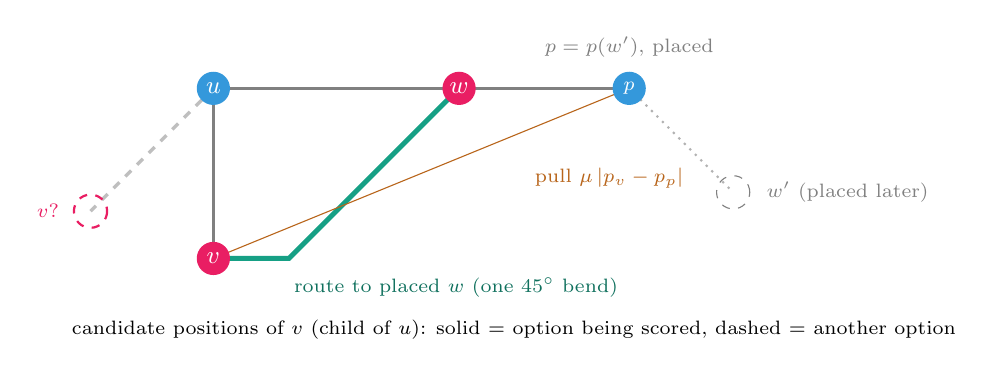
\begin{tikzpicture}[yscale=-1, scale=1.2, >=Stealth]
% committed tree links
\coordinate (u) at (0,0); \coordinate (w) at (2.6,0); \coordinate (p) at (4.4,0);
\coordinate (v1) at (0,1.8); \coordinate (v2) at (-1.3,1.3); \coordinate (wp) at (5.5,1.1);
\draw[very thick, gray] (u) -- (w) -- (p);
\draw[very thick, gray] (u) -- (v1);
\draw[very thick, gray!50, dashed] (u) -- (v2);
% cycle edge from v to the placed neighbour w: one 45-degree bend
\draw[line width=1.8pt, cyc] (v1) -- (0.8,1.8) -- (w);
\node[font=\scriptsize, cyc!70!black, anchor=north west] at (0.75,1.9) {route to placed $w$ (one $45^\circ$ bend)};
% pull towards the parent of the not-yet-placed neighbour w'
\draw[<->, thin, hot!80!black] (v1) -- (p);
\node[font=\scriptsize, hot!80!black, anchor=west] at (3.3,0.95) {pull $\mu\,|p_v-p_{p}|$};
% future w'
\draw[gray!60, dotted, thick] (p) -- (wp);
\node[draw, dashed, circle, minimum size=12pt, inner sep=0, gray] at (wp) {};
\node[font=\scriptsize, gray, anchor=west] at ($(wp)+(0.25,0)$) {$w'$ (placed later)};
\node[font=\scriptsize, gray, anchor=south] at ($(p)+(0,-0.22)$) {$p=p(w')$, placed};
\fill[male] (u) circle (5pt); \node[white, font=\small] at (u) {$u$};
\fill[female] (w) circle (5pt); \node[white, font=\small] at (w) {$w$};
\fill[male] (p) circle (5pt); \node[white, font=\scriptsize] at (p) {$p$};
\fill[female] (v1) circle (5pt); \node[white, font=\small] at (v1) {$v$};
\draw[female, thick, dashed] (v2) circle (5pt); \node[font=\scriptsize, female] at ($(v2)+(-0.45,0)$) {$v$?};
\node[font=\scriptsize, anchor=west] at (-1.6,2.55) {candidate positions of $v$ (child of $u$): solid = option being scored, dashed = another option};
\end{tikzpicture}
\caption{Scoring one candidate position of $v$ (child of $u$). The cycle edge to the placed neighbour $w$ is routed immediately (green) and its cost is added. The not-yet-placed cycle neighbour $w'$ will be placed next to its BFS parent $p$, so the distance from $v$ to $p$ is added as a pull. Unplaced neighbours whose parent is not placed yet contribute nothing.}
\label{fig:expand}
\end{figure}

\begin{algorithm}[ht]
\caption{\textsc{Expand} with cycle edges (for child $v$ of $u$; beam $\mathcal B$, options $O$)}
\label{alg:expand}
\begin{algorithmic}[1]
\ForAll{states $S\in\mathcal B$}
  \State $\mathit{used}\gets \mathit{usedPorts}(u)\ \cup$ \{back direction of $u$\} $\cup$ \{first directions of the children in $S$\}
  \ForAll{options $o\in O$ with first direction $\notin \mathit{used}$}
     \State place $v$ by $o$ (tree link, as in the tree algorithm); $\ c\gets\Score_{\text{tree}}(o)$; $\ \mathit{own}\gets$ tree-link segments
     \ForAll{cycle neighbours $w$ of $v$}
        \If{$w$ is placed (committed or in $S$)}
           \State $R\gets$ cheaper of the shapes of $w$--$v$ (\cref{sec:routecost}), checked against committed geometry, $S$ and $\mathit{own}$
           \State $c\gets c+\operatorname{cost}(R)$; $\ \mathit{own}\gets\mathit{own}\cup R$
        \ElsIf{$p(w)$ is placed} \State $c\gets c+\mu\,|p_v-p_{p(w)}|$ \EndIf
     \EndFor
     \State add $(S\cup\{(o,\text{routes})\},\ \mathrm{cost}(S)+c)$ to the result
  \EndFor
\EndFor
\State if no option had a free direction, repeat without the direction test (the conflict is then penalised as an edge collision)
\end{algorithmic}
\end{algorithm}

When the best state is committed, the cycle edges stored with it become part of the drawing: their segments are added to the list of drawn segments (so every later placement avoids them) and their bends are stored for drawing.

\subsection{Port reservation}
\label{sec:ports}

For every placed vertex the algorithm keeps the set $\mathit{usedPorts}(x)$ of directions already used at $x$: the arriving tree link, the links to its children and the ends of its cycle edges. When the children of $u$ are placed, every direction in $\mathit{usedPorts}(u)$ is blocked for their first segments, exactly like the back direction in the tree algorithm. In particular, if a cycle edge reached $u$ after $u$ was placed but before its children were, the children avoid that direction. For a tree, $\mathit{usedPorts}(u)$ contains only the arriving direction, so nothing changes. The ports of cycle edges themselves cannot be chosen freely (they follow from the geometry), so conflicts at their endpoints are penalised through $E_r$ rather than forbidden.

%==========================================================================
\section{Several components}
\label{sec:components}

Each connected component is laid out on its own, from the root for the root's component and from its first vertex for the others. The drawings are then placed from left to right in that order: each component is shifted so that its leftmost point is 120\,px to the right of everything drawn so far, and its top is aligned with the top of the drawing so far (\cref{fig:disc}). The BFS layer display and the step-by-step order merge the components layer by layer (layer $d$ holds every vertex at depth $d$ in its own component). For a connected graph nothing is shifted, so the layout is unchanged.

\begin{figure}[ht]
\centering
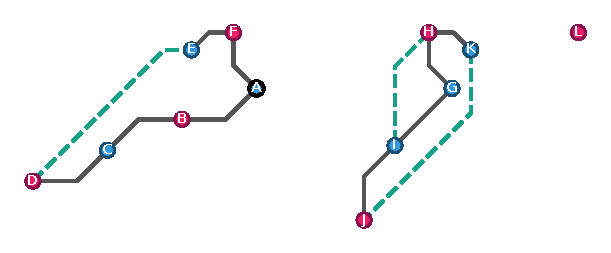
\includegraphics[width=0.62\textwidth]{fig_disc.pdf}
\caption{A graph with three components: a 6-cycle (root A), a 5-vertex component with two cycles, and an isolated vertex L.}
\label{fig:disc}
\end{figure}

%==========================================================================
\section{Settings search}
\label{sec:search}

The layout has three global settings: the starting edge length $L_0$ (90\,px for up to 100 vertices, then $+30$\,px per further band of 25 vertices), the beam width $B$, and an optional extra shrink per generation (effective $\alpha$ is the user's $\alpha$ times a factor). The search runs whenever the graph has a cycle (and, as in the tree version, for trees with more than 100 vertices). It tries candidate settings in five stages and keeps the layout with the fewest overlapping vertex pairs, then the fewest colliding edge pairs:

\begin{center}\small
\begin{tabular}{@{}c l@{}}
\toprule
extra shrink & candidates (length factor $f$ times $L_0$, beam width $B$), shortest first\\
\midrule
$\times1$ (user's $\alpha$) & $(1,4)$, $(1,1)$, $(1,2)$, $(1.25,2)$, $(1.5,2)$, $(1.75,2)$, $(2,1)$, $(2.5,1)$, $(3,2)$\\
$\times0.8$ & $(1.5,2)$, $(1.75,2)$, $(3,1)$, $(3,2)$\\
$\times0.7$ & $(1.25,1)$, $(1.5,1)$, $(1.75,1)$\\
$\times0.6$ & $(2,1)$, $(2.5,1)$, $(2.5,2)$\\
$\times0.5$ & $(2,1)$, $(2.5,2)$, $(3,1)$, $(3,2)$\\
\bottomrule
\end{tabular}
\end{center}

The search stops at the first candidate without any overlap. Because the default setting $(1,4)$ is tried first, the result is never worse than a single run, the user's $\alpha$ is kept whenever that is enough, and among clean layouts the most compact one is chosen. Vertex overlaps are counted with a threshold of 17.5\,px in the search (16\,px plus the effect of rounding positions to whole pixels on screen). The chosen setting is cached per graph, root and $\alpha$, so Run Full Metro Layout, Step by Step BFS Draw, the overlap panels and the Fix buttons all use the same layout; the status line reports which setting was used.

%==========================================================================
\section{Overlap detection}
\label{sec:detect}

\begin{itemize}
  \item \textbf{Vertex overlaps:} two visible vertices whose on-screen positions are closer than 16\,px (the disk size).
  \item \textbf{Edge collisions:} every pair of segments of different edges (tree or cycle) is tested. Two segments collide if they cross, if they leave a shared endpoint in the same direction (angle difference below $0.05$\,rad), or if they come closer than 6\,px without sharing an endpoint. Segments of the same edge are never compared.
\end{itemize}
Pairs are grouped into connected components, so that mutually overlapping vertices or edges are listed once (``Vertices B, H, N overlap'', ``Edges A-B, B-C collide / overlap''). A group of edges is reported as \emph{collide / overlap} if at least one of its pairs crosses or shares a start direction, and as \emph{touch} otherwise. Groups are listed in a fixed order: by their first member, with vertices in input order and edges in alphabetical order, and the members of a group in the same order.

\subsection{Incremental checking in Step by Step BFS Draw}
\label{sec:incremental}

Step by Step BFS Draw computes the complete layout once, on its first click, and then reveals one vertex per click in BFS order. The overlap lists must show exactly what the full check would report for the part drawn so far, and mark groups that appeared in the last click as NEW. Recomputing them from scratch after every click (all vertex pairs, all segment pairs, and in the earlier version even the layout itself) costs $O(n^2)$ per click and $O(n^3)$ for a click-through. They are therefore updated incrementally:

\begin{enumerate}
  \item \textbf{Stored data (first click).} The whole-pixel screen position of every vertex, the segments of every edge with their index in the segment list, and for every vertex the edges incident to it.
  \item \textbf{New vertex.} When vertex $x$ is revealed it is compared with the vertices already drawn only: $O(n)$.
  \item \textbf{New edges.} The edges that become visible are the edges from $x$ to drawn vertices (at most $\deg x\le 8$). Each is compared with the edges already drawn only, $O(m)$ per click. For a pair of edges the segment pairs (at most 4) are tested in the order of the full check (by index in the segment list), so the first colliding pair gives the same \emph{touch} / \emph{overlap} type.
  \item \textbf{Groups.} Overlapping vertices and colliding edges are kept in two union-find structures (union by size, path compression). Every group stores its members sorted in the listing order (two groups are merged by a linear merge of their sorted lists), the sums of the vertex coordinates (for the ``overlap at approx $(x,y)$'' position) and whether it contains a real overlap. Because vertices and edges are only ever added and positions never change, groups only grow or merge and never split.
  \item \textbf{NEW.} A group is new in a click exactly when it was created or grew in that click, so the groups touched by the unions of the click are marked; no comparison with the previous lists is needed.
  \item \textbf{Listing.} The lists are written by one pass over all vertices and one pass over all edges in listing order, printing each group at its first member: $O(n+m)$ per click.
\end{enumerate}

\noindent The lists produced this way were compared with the old implementation after every click in 15 runs on 14 graphs (679 clicks, including graphs with up to 6 groups of overlapping vertices and 5 groups of colliding edges): members, types, positions and NEW marks were identical in every click.

%==========================================================================
\section{Overlap repair (The Fix buttons)}
\label{sec:fix}

\subsection{Prevention during the layout}
Most overlaps are prevented while the layout is built, by the terms of the placement score: vertex conflicts ($10^6$) and edge conflicts ($10^5$) of tree links, the same two terms for every routed cycle edge, the pull towards future cycle neighbours, port reservation, and finally the settings search, which compares complete layouts.

\subsection{The Fix buttons}
The two buttons run a local search over \emph{overrides}: choices that the layout must respect when it is run again.
\begin{itemize}
  \item a forced branch offset $g$ and/or bend sign $s$ for one tree link (the paper's ``flipping of sub-trees'');
  \item a length factor (0.76--1.3) for one tree link;
  \item a local shrinking factor (0.8, 0.65 or 0.5) for the subtree below a vertex (a local version of Lemma 4.3 of Korst et al.).
\end{itemize}
After each change the whole layout is re-run, so the vertices below the modified link move and \textbf{all cycle edges are re-routed} with the rules of \cref{sec:cycle}; cycle edges therefore never need overrides of their own.

\begin{algorithm}[ht]
\caption{\textsc{Fix}(mode), mode $\in\{$vertex, edge$\}$}
\label{alg:fix}
\begin{algorithmic}[1]
\State $\mathit{best}\gets$ current overrides; $e\gets\textsc{Evaluate}(\mathit{best})$
\For{at most 16 rounds, while overlaps of this kind remain and the budget is not used up}
  \State $\mathcal C\gets$ vertices involved in the overlaps (vertex mode), or the child end of every colliding tree edge and \textbf{both ends of every colliding cycle edge} (edge mode); add their BFS parents and grandparents
  \ForAll{$x\in\mathcal C$ with parent $p$} try every $(g,s)$ for link $p\to x$; keep the best if it lowers the cost \EndFor
  \If{nothing improved} try length factors for one link \EndIf
  \If{nothing improved} try local shrinking of one subtree \EndIf
  \If{nothing improved} \textbf{stop} \EndIf
\EndFor
\end{algorithmic}
\end{algorithm}

\textsc{Evaluate} runs the layout and returns
\[
  \mathrm{cost}=100\,000\cdot(\#\text{vertex overlaps})+5\,000\cdot(\#\text{colliding edge pairs})-(\text{minimum vertex distance}).
\] Fix Edge Overlaps never accepts a change that adds vertex overlaps. The number of evaluations is limited to $\max(150,\min(500,\lfloor 25\,000/n\rceil))$. Every accepted change is listed in Summary of Changes; overlaps that remain are listed in red. \Cref{fig:tc80} shows the effect on a tree with additional cycle edges.

\begin{figure}[ht]
\centering
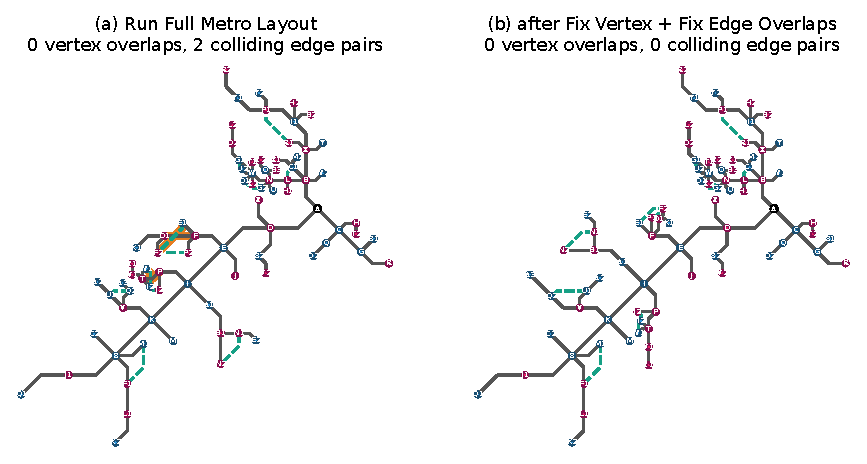
\includegraphics[width=0.95\textwidth]{fig_tc80.pdf}
\caption{An 80-vertex tree with 12 additional cycle edges ($\alpha=0.75$). (a) After Run Full Metro Layout two pairs of edges collide (orange). (b) The Fix buttons re-route the affected links and remove both collisions.}
\label{fig:tc80}
\end{figure}

\subsection{What cannot be fixed}
\begin{itemize}
  \item crossings forced by non-planarity (\cref{sec:planarity});
  \item a vertex whose required directions exceed the free ones (eight in total, seven at a non-root vertex besides its parent edge);
  \item crossings that would need a change outside the search space of the fixers, e.g.\ moving a single vertex independently of its subtree, or choosing a different spanning tree.
\end{itemize}

%==========================================================================
\section{Time and space complexity}
\label{sec:complexity}

Let $n$ be the number of vertices and $m$ the number of edges. The degree bound gives $m\le 4n$, the drawing has at most $2m\le 8n$ segments, and there are $k=m-n+c\le m$ cycle edges. The beam width $B\le4$ and the number of options per child $|O|\le12$ are constants.

\begin{enumerate}
  \item \textbf{Checks and spanning forest:} degree check, BFS forest and cycle-edge classification take $O(n+m)$.
  \item \textbf{Tree links:} as in the tree algorithm, each of the $n-c$ children is evaluated in $B|O|$ candidates; a candidate is checked against the geometry near its parent and its average distance to all placed vertices is computed, $O(n+m)$ per candidate. Total $O(B|O|\,n(n+m))=O(n^2)$.
  \item \textbf{Cycle edges:} a cycle edge is routed in every candidate of its second endpoint, at most $B|O|$ times, with 2 shapes, each checked against all placed vertices and all drawn segments, $O(n+m)$. Total $O(B|O|\,k\,(n+m))=O(n^2)$ since $k\le m\le 4n$. The pull term costs $O(\deg v)$ per candidate.
  \item \textbf{One layout:} $O\bigl(B|O|\,(n+k)(n+m)\bigr)=O(n^2)$ time and $O(n+m)=O(n)$ space (positions, bends, segments, port sets; the beam holds at most $B|O|$ partial assignments of one vertex's children).
  \item \textbf{Quality evaluation:} all vertex pairs and all segment pairs, $O(n^2+m^2)=O(n^2)$ (most segment pairs are rejected by a bounding-box test in constant time).
  \item \textbf{Settings search:} at most 23 layouts with their evaluations, $O(n^2)$ with a constant factor of at most 23; afterwards the result is cached.
  \item \textbf{Step by Step BFS} (\cref{sec:incremental}): the first click computes the layout, $O(n^2)$ (the settings search is cached if the layout was run before). Every further click compares the new vertex with the drawn vertices, $O(n)$, and its at most 8 new edges (at most 2 segments each) with the drawn segments, $O(m)$, and rewrites both lists, $O(n+m)$; redrawing the visible edges is $O(m)$. Merging groups costs time linear in their sizes; since there are at most $n-1$ merges of vertex groups and $m-1$ of edge groups, each of cost at most $n$ resp.\ $m$, all merges of a run together cost $O(n^2+m^2)$. A complete click-through therefore takes $O(n\cdot(n+m)+n^2+m^2)=O(n^2)$ time, the same order as Run Full Metro Layout, and $O(n+m)$ space. (Recomputing the lists from scratch after every click, as in the first version, costs $\Theta(k^2)$ in click $k$ and $\sum_k k^2=\Theta(n^3)$ in total.)
  \item \textbf{Fix buttons:} at most $\max(150,\min(500,25\,000/n))$ evaluations of $O(n^2)$ each, i.e.\ $O(n^2)$ with a large constant (and $O(n)$ space per stored set of overrides).
\end{enumerate}

\begin{table}[ht]
\centering\footnotesize
\setlength{\tabcolsep}{4pt}
\begin{tabular}{@{}l r r r l@{}}
\toprule
graph & $n$ & $m$ & time & environment\\
\midrule
grid $5\times5$ & 25 & 40 & 59\,ms & Chromium, Run Full Metro Layout\\
random graph, degree $\le4$ & 40 & 52 & 159\,ms & Chromium\\
tree with cycle edges & 80 & 91 & 314\,ms & Chromium\\
tree with cycle edges & 300 & 344 & 2.3\,s & Chromium\\
tree with cycle edges & 150 / 220 / 300 & & 0.8 / 1.4 / 2.1\,s & Node.js, incl.\ settings search\\
grid $12\times12$ / $17\times17$ & 144 / 289 & 264 / 544 & 1.2 / 5.3\,s & Node.js\\
Fix Vertex + Fix Edge, random graph & 40 & 52 & 2.4\,s & Chromium\\
\bottomrule
\end{tabular}
\caption{Measured running times of the first layout of a graph (including the settings search) and of the Fix buttons.}
\label{tab:time}
\end{table}

\begin{table}[ht]
\centering\footnotesize
\begin{tabular}{@{}r r r r r@{}}
\toprule
$n$ (tree with cycle edges) & $m$ & recomputing the lists ($O(n^3)$) & incremental ($O(n^2)$) & speed-up\\
\midrule
80 & 91 & 1.3\,s & 0.17\,s & $8\times$\\
150 & 172 & 5.5\,s & 0.56\,s & $10\times$\\
220 & 252 & 21.2\,s & 1.7\,s & $12\times$\\
300 & 344 & 38.4\,s & 2.3\,s & $17\times$\\
\bottomrule
\end{tabular}
\caption{Time for a complete Step by Step BFS click-through after the first click (Chromium, $\alpha=0.75$): the earlier version, which recomputed the layout and all pairs after every click, and the incremental version. The ratio grows roughly linearly with $n$, as expected from $O(n^3)$ against $O(n^2)$.}
\label{tab:steptime}
\end{table}

%==========================================================================
\section{Experiments}
\label{sec:experiments}

Five sets of test graphs were laid out with root A: 12 trees with about 15\% additional edges between vertices at BFS distance 2--3 ($n=20,40,80,150$, at most 3 children per vertex); 6 grids from $3\times3$ to $10\times12$; the cycles $C_5,C_6,C_{12},C_{30},C_{60}$; 6 random graphs with degree $\le4$ ($n=20,40,80$, $m\approx1.3n$); and 4 random graphs with degree $\le8$ ($n=30,60$, $m\approx1.8n$). The graphs are provided as \texttt{graph\_experiment\_sets.zip} (adjacency lists, with an index of their sizes and results). The experiment used each vertex's neighbours in the order in which the generator created them; the page's list importer builds the neighbour lists in a different order, which changes the BFS spanning tree slightly, so per-graph results after importing a file can differ a little from the table (for example 39 instead of 44 colliding edge pairs for the first set at $\alpha=0.75$); the index lists both. Three variants are compared: \emph{naive} (cycle edges routed, but their route cost is not added to the placement score; the pull is kept; no settings search), \emph{no search} (cycle-aware placement, single run) and the \emph{final} algorithm.

\begin{table}[H]
\centering\footnotesize
\setlength{\tabcolsep}{4pt}
\begin{tabular}{@{}l c ccc@{}}
\toprule
set & $\alpha$ & naive & no search & final\\
\midrule
\multirow{3}{*}{trees + cycle edges (12)} & 1.0 & 0/140 (2) & 0/65 (3) & 0/39 (4)\\
 & 0.75 & 8/126 (1) & 4/75 (2) & 0/44 (3)\\
 & 0.5 & 17/133 (2) & 15/77 (3) & 0/45 (3)\\
\midrule
\multirow{3}{*}{grids (6)} & 1.0 & 0/497 (0) & 0/0 (6) & 0/0 (6)\\
 & 0.75 & 0/944 (0) & 0/3 (4) & 0/0 (6)\\
 & 0.5 & 0/707 (0) & 1/51 (3) & 0/0 (6)\\
\midrule
\multirow{3}{*}{cycles (5)} & 1.0 & 0/0 (5) & 0/0 (5) & 0/0 (5)\\
 & 0.75 & 0/3 (2) & 0/0 (5) & 0/0 (5)\\
 & 0.5 & 0/3 (2) & 0/0 (5) & 0/0 (5)\\
\midrule
\multirow{3}{*}{random, degree $\le 4$ (6)} & 1.0 & 0/429 & 0/334 & 0/178\\
 & 0.75 & 2/325 & 5/267 & 0/178\\
 & 0.5 & 6/369 & 2/340 & 0/192\\
\midrule
\multirow{3}{*}{random, degree $\le 8$ (4)} & 1.0 & 0/1188 & 0/881 & 0/611\\
 & 0.75 & 3/1044 & 4/1142 & 0/676\\
 & 0.5 & 17/1072 & 21/986 & 1/686\\
\bottomrule
\end{tabular}
\caption{Overlapping vertex pairs / colliding edge pairs, summed over each set, and in brackets the number of graphs drawn without any overlap (random graphs: none in any variant). Every edge in every layout was checked to be straight or to have exactly one $45^\circ$ bend.}
\label{tab:exp}
\end{table}

\begin{figure}[H]
\centering
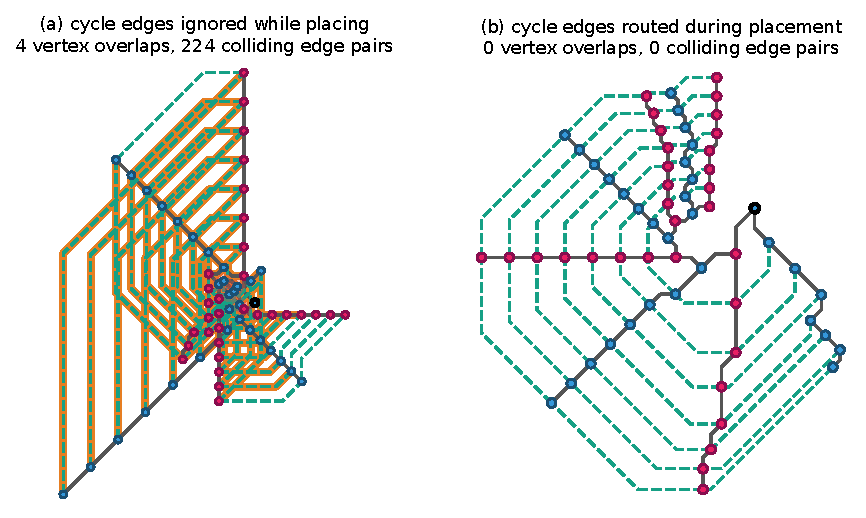
\includegraphics[width=0.95\textwidth]{fig_grid8.pdf}
\caption{An $8\times8$ grid ($n=64$, $m=112$, 49 cycle edges), $\alpha=0.75$. (a) If cycle edges are ignored while the vertices are placed (no route cost, no pull, no settings search) and only drawn afterwards, the BFS tree spreads the grid out and the cycle edges collide massively (orange). (b) With the route cost and the pull in the placement score the grid is drawn without any overlap.}
\label{fig:grid8}
\end{figure}

Observations: routing cycle edges during placement is the decisive step (grids: hundreds of collisions become none); the settings search removes the remaining vertex overlaps and lowers edge collisions further, especially for small $\alpha$. Random graphs keep collisions: many of them are not planar, and the spanning-tree-first strategy cannot rearrange the drawing globally. The Fix buttons improve them further (e.g.\ 15 to 6 colliding edge pairs on a 40-vertex random graph).

%==========================================================================
\section{Limitations}

\begin{itemize}
  \item \textbf{Heuristic.} The method gives no guarantee of a crossing-free drawing even for planar graphs and does not minimise the number of crossings; non-planar graphs keep at least $\operatorname{cr}(G)$ crossings.
  \item \textbf{Fixed spanning tree.} The BFS tree from the chosen root decides which edges are tree links; another root or another spanning tree can give a better drawing.
  \item \textbf{Cycle edges have free lengths.} Their length is set by their endpoints, not by $\alpha$; the gender rule applies to tree links only.
  \item \textbf{Ports of cycle edges} follow from the geometry; with many cycle edges at one vertex, direction conflicts are possible even when $\deg\le8$.
  \item \textbf{Size.} The page draws at most 300 vertices; the first layout of a large graph with cycles can take a few seconds.
\end{itemize}

\vspace{1em}
\noindent\textbf{Reference.} J.~Korst, V.~Pronk and J.~J.~van Wijk. A Visualization of Family Relations Inspired by the London Metro Map. In \emph{VINCI 2020}, Eindhoven, The Netherlands. ACM, 2020. \url{https://doi.org/10.1145/3430036.3430065}

\end{document}
